\documentclass[conference]{IEEEtran}
\usepackage{cite}
\usepackage{amsmath,amsthm}
\usepackage{newtxtext,newtxmath}
\usepackage{graphicx}
\usepackage{booktabs}
\usepackage{multirow}
\usepackage{tikz}
\usetikzlibrary{positioning,arrows.meta}
\usepackage{xcolor}
\usepackage{url}
\usepackage[hidelinks]{hyperref}

\graphicspath{{../../results/figures/paper/}}

\newtheorem{proposition}{Proposition}
\theoremstyle{definition}
\newtheorem{definition}{Definition}

\newcommand{\A}{A(a)}
\newcommand{\Sib}{S(a)}
\newcommand{\anc}{\mathrm{anc}}
\newcommand{\full}{\mathrm{full}}
\newcommand{\win}{\mathrm{win}}
\newcommand{\todo}[1]{\textcolor{red}{\textbf{[TODO: #1]}}}

\definecolor{ancblue}{HTML}{2A78D6}
\definecolor{sibor}{HTML}{EB6834}
\definecolor{offgray}{HTML}{C3C2B7}

\begin{document}

\title{The Only Path That Matters? Ancestor-Only Context Selection in Branched LLM Conversations}

\author{\IEEEauthorblockN{Okechukwu Zeal Achonu}
\IEEEauthorblockA{Department of Mathematics and Computer Science\\
Fisk University, Nashville, TN, USA\\
okechukwuzealachonu@gmail.com}}

\maketitle

\begin{abstract}
Large language models (LLMs) are increasingly used for exploratory programming, in which a user tries several implementation paths before settling on one. Because linear chat interfaces keep every abandoned path in the context window, each new turn re-sends material that no longer matters, which raises token cost and can make the model less reliable as the dialogue grows. Branching interfaces avoid this by sending the model only the active root-to-node path. Prior evaluations, however, compared that rule only against the full linear history, so they could not tell whether its benefit came from a better-chosen context or simply a shorter one. This paper separates the two by evaluating ancestor-only prompting in Traceback, a chat platform that stores conversations as trees and retrieves the active path with a recursive common table expression. On a frozen benchmark of 720 synthetic branched conversations that vary depth, sibling count, sibling type, sibling recency and the position of the required fact, three LLMs answered a final question under three context rules: ancestor-only, full-tree concatenation, and a sliding window capped at the ancestor-only token budget. Ancestor-only prompting used 62.7\% fewer input tokens than the full tree, produced no sibling leakage in 2{,}160 answers (exact 95\% upper bound 0.17\%), and was correct in 99.9\% of cases. The full tree was nearly as accurate (98.6\%) but paid in tokens, leakage and judged quality, whereas the equal-budget window was correct in only 52.0\% of cases. A short formal analysis explains why: it predicts the token savings exactly and shows that a recency window must discard root-side facts, and every prediction held in all 720 scenarios. The one measurable cost of ancestor-only prompting arises with consistent siblings, whose details can recover a fact that a recency window has dropped.
\end{abstract}

\begin{IEEEkeywords}
large language models, context management, branched conversations, prompt construction, context window, evaluation
\end{IEEEkeywords}

\section{Introduction}

LLMs are now widely used in exploratory programming, where a developer often tries several implementation paths before settling on one. In a conventional chat transcript, every one of those abandoned paths stays in the context window, so each new turn re-sends tangents that no longer matter. The cost of this grows with the conversation, and so does the risk to the answer: long, noisy context is known to make models less reliable \cite{hong2025contextrot,liu2024lost}.

Branching interfaces address the problem by treating a conversation as a tree rather than a list. A user can branch from any earlier message to explore an alternative, and when they continue on one branch, the model is sent only the path from the root to the current message. Traceback, the platform used in this work, implements this by storing each message as a database row linked to its parent and retrieving the path with a recursive common table expression (CTE). We refer to this rule as \emph{ancestor-only prompting}.

Ancestor-only prompts are shorter than the full history, so a natural question is whether their advantage comes from length alone. This paper therefore asks whether, at an equal token budget, selecting context by tree structure rather than by recency reduces \emph{sibling leakage}, that is, the model using facts from inactive branches. It further asks how leakage varies with the kind of content a sibling holds, and whether answer quality on the active path is preserved. We hypothesize that ancestor-only prompting uses fewer tokens than full-tree concatenation, that both baselines show measurable sibling leakage, and that answer quality is preserved whenever the needed context lies on the active path.

To test these claims, this paper makes four contributions:
\begin{itemize}
  \item a benchmark of 720 branched conversations with controlled sibling types (consistent, conflicting, irrelevant, misleading), recency and fact position, frozen and hashed before any model call;
  \item a comparison of ancestor-only prompting against an equal-budget sliding window, with full-tree concatenation as a reference, on three models from different families;
  \item a short formal framework whose predictions about token efficiency and window displacement are checked scenario by scenario; and
  \item leakage rates reported per sibling type that separate answers which \emph{use} a sibling detail from answers which only mention or reject it.
\end{itemize}
The study is limited to text-only, synthetic dialogues, and semantic retrieval across branches is left to future work.

\section{Related Work}

\textit{Long context.} The case for pruning context rests on evidence that models degrade as their input grows. Hong et al.\ \cite{hong2025contextrot} tested 18 frontier models and found that performance became less reliable as input length increased, even on simple tasks and well below each model's context limit. Liu et al.\ \cite{liu2024lost} showed, in addition, that models use information best when it sits at the start or end of a long input and worst when it sits in the middle. An abandoned exploration adds exactly this kind of irrelevant length, and it pushes earlier relevant turns towards the middle of the prompt.

\textit{Context reduction.} Several methods already shorten prompts in linear dialogues. Sliding windows keep only the most recent turns, while summarization and prompt compression methods such as LongLLMLingua \cite{jiang2024longllmlingua} condense the history. All of them, however, select context by position or by estimated importance, and none of them use the branch structure of a conversation.

\textit{Branching.} Work on branched conversations has begun to fill that gap. Hemanth and Saha \cite{hemanth2026cta} describe how topically distinct threads in a flat, append-only window bleed into one another, and they formalize context-isolated tree nodes, although without a controlled comparison against other context strategies. Chickmagalur Nanjundappa and Maaheshwari \cite{nanjundappa2025branching} did run such a comparison: across 30 software engineering scenarios, branching cut context size by 58.1\% while improving response quality. Their branched condition is in effect ancestor-only prompting and their linear condition is full-tree concatenation. Because the study had no length-matched condition, however, it cannot show whether the advantage survives when length is held fixed.

No prior work, then, compares ancestor-only context against an equal-budget window or measures leakage by sibling type. This paper addresses both.

\section{Framework and Experimental Platform}

\subsection{Definitions}

To reason about the three rules precisely, we model a session as a rooted tree $T=(V,E)$ of messages with root $r$ and parent map $p$. A logical clock $\tau$ assigns each message a distinct time that increases along every edge, so a reply is always newer than the message it answers. Each message also has a token weight $w(v)>0$ under a fixed reference tokenizer, and for a set of messages $U\subseteq V$ we write $w(U)=\sum_{u\in U}w(u)$. The user asks a question $q$ as a child of an ask node $a$, later than every existing message. The active path is then $\A=\{a,p(a),\dots,r\}$, and everything else, $\Sib=V\setminus\A$, is sibling content.

\begin{definition}[Context rules]
Ancestor-only: $C_\anc=\A$, ordered root to node. Full tree: $C_\full=V$, ordered by $\tau$. Sliding window: $C_\win$ is the longest run of newest messages whose total weight is at most $B=w(\A)$, never splitting a message.
\end{definition}

The window's budget is set equal to the size of the ancestor-only prompt, so the two rules always send the same amount of text and differ only in how they choose it. Fig.~\ref{fig:rules} shows the three rules on a small tree.

\begin{figure*}[t]
\centering
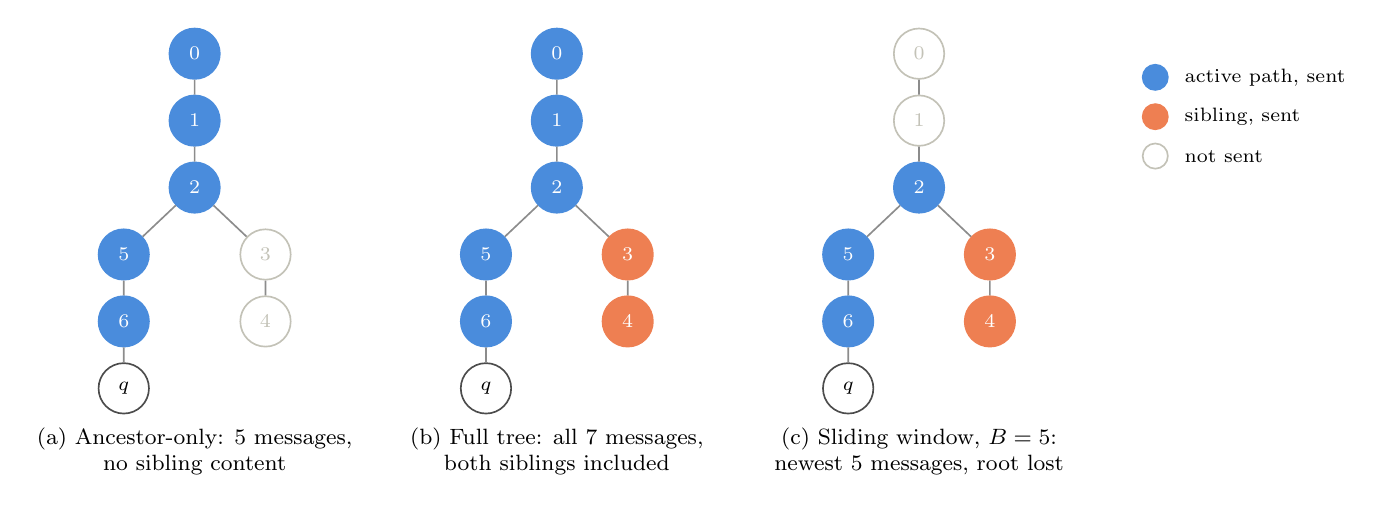
\begin{tikzpicture}[
  msg/.style={circle, draw, minimum size=6.4mm, inner sep=0pt, font=\scriptsize, line width=0.6pt},
  on/.style={msg, fill=ancblue!85, draw=ancblue!85, text=white},
  sib/.style={msg, fill=sibor!85, draw=sibor!85, text=white},
  off/.style={msg, draw=offgray, text=offgray, fill=white},
  q/.style={msg, draw=black!70, text=black, fill=white},
  edge/.style={-, line width=0.6pt, color=black!45},
  lab/.style={font=\footnotesize, align=center}]
\newcommand{\tree}[8]{%
  \begin{scope}[shift={(#1,0)}]
    \node[#2] (r) at (0,0) {0};
    \node[#3] (m) at (0,-0.85) {1};
    \node[#4] (f) at (0,-1.7) {2};
    \node[#5] (s1) at (0.9,-2.55) {3};
    \node[#6] (s2) at (0.9,-3.4) {4};
    \node[#7] (a1) at (-0.9,-2.55) {5};
    \node[#8] (a) at (-0.9,-3.4) {6};
    \node[q] (qq) at (-0.9,-4.25) {$q$};
    \draw[edge] (r)--(m) (m)--(f) (f)--(s1) (s1)--(s2) (f)--(a1) (a1)--(a) (a)--(qq);
  \end{scope}}
\tree{0}{on}{on}{on}{off}{off}{on}{on}
\tree{4.6}{on}{on}{on}{sib}{sib}{on}{on}
\tree{9.2}{off}{off}{on}{sib}{sib}{on}{on}
\node[lab] at (0,-5.05) {(a) Ancestor-only: 5 messages,\\no sibling content};
\node[lab] at (4.6,-5.05) {(b) Full tree: all 7 messages,\\both siblings included};
\node[lab] at (9.2,-5.05) {(c) Sliding window, $B=5$:\\newest 5 messages, root lost};
\node[on, minimum size=3.2mm] at (12.2,-0.3) {}; \node[font=\scriptsize, anchor=west] at (12.45,-0.3) {active path, sent};
\node[sib, minimum size=3.2mm] at (12.2,-0.8) {}; \node[font=\scriptsize, anchor=west] at (12.45,-0.8) {sibling, sent};
\node[off, minimum size=3.2mm] at (12.2,-1.3) {}; \node[font=\scriptsize, anchor=west] at (12.45,-1.3) {not sent};
\end{tikzpicture}
\caption{The three context rules on one session. Numbers give the logical clock $\tau$; messages 3--4 are a sibling branch explored before the active path continued. With equal message weights the window budget is $B=w(\A)=5$, so the window keeps the five newest messages and drops the root, as Proposition~\ref{prop:window} requires.}
\label{fig:rules}
\end{figure*}

\subsection{Propositions}

Six short propositions follow from these definitions. The first two concern cost, the next two concern what can leak, and the last two explain what the window must discard.

\begin{proposition}[Efficiency]\label{prop:eff}
$C_\anc\subseteq C_\full$, and the token efficiency equals the siblings' share of the tree:
\[E=1-\frac{w(C_\anc)}{w(C_\full)}=\frac{w(\Sib)}{w(V)}.\]
\end{proposition}
\begin{proof}
$\A\subseteq V$ and $w$ is a sum of positive terms. Since $V=\A\,\dot\cup\,\Sib$, $w(V)=w(\A)+w(\Sib)$, which rearranges to the formula.
\end{proof}

Proposition~\ref{prop:eff} turns the token saving into arithmetic on the tree, so it can be known before any model is called. Over a whole session the gap widens further, because the full tree is re-sent and grows on every turn:

\begin{proposition}[Growth]\label{prop:growth}
If a session grows one message at a time, each step re-sends its context, weights lie in $[w_{\min},w_{\max}]$ and the answered depth is at most $D$, the cumulative full-tree cost is at least $w_{\min}n(n+1)/2=\Theta(n^2)$, while the cumulative ancestor-only cost is at most $w_{\max}n(D+1)=O(nD)$.
\end{proposition}
\begin{proof}
$|V_t|=t$ gives $w(V_t)\ge tw_{\min}$; a root-to-node path at depth $d_t\le D$ has $d_t+1$ messages.
\end{proof}

The cost advantage is therefore guaranteed by construction. Whether sibling content can reach the answer is a separate question, and here too ancestor-only prompting has a structural guarantee:

\begin{proposition}[No sibling facts]\label{prop:nosib}
If every message containing a fact $f$ lies in $\Sib$ and $q$ does not contain $f$, then $f$ is absent from the ancestor-only prompt.
\end{proposition}
\begin{proof}
That prompt is the text of $\A$ followed by $q$, and $\A\cap\Sib=\varnothing$.
\end{proof}

A sibling-only fact can therefore appear in an ancestor-only answer only by chance. For the other rules, leakage depends both on whether the fact reached the prompt and on what the model did with it, which the next proposition separates.

\begin{proposition}[Exposure and uptake]\label{prop:decomp}
Let $X_c(f)$ indicate that $f$ is in the prompt of rule $c$, $\pi_f$ the rate of mentioning $f$ without seeing it, and $u_c(f)$ the rate when exposed. $X_c(f)$ is a function of $(T,\tau,w,a)$ alone, and for a sibling-only fact
\[\Pr(M\mid c)-\Pr(M\mid\anc)=X_c(f)\,\bigl(u_c(f)-\pi_f\bigr).\]
\end{proposition}
\begin{proof}
By Proposition~\ref{prop:nosib}, $\Pr(M\mid\anc)=\pi_f$; under rule $c$ the rate is $\pi_f$ if $X_c(f)=0$ and $u_c(f)$ otherwise.
\end{proof}

This decomposition is why leakage is measured as an excess over the ancestor-only rate, and why the experiment logs exposure for every call. Exposure can be computed from the tree alone, so the role of the models is reduced to uptake. For the window in particular, exposure is fully determined by which messages it keeps, which the last two propositions characterize.

\begin{proposition}[Window membership]\label{prop:window}
A message $m$ is in $C_\win$ if and only if $\sum_{u:\,\tau(u)\ge\tau(m)}w(u)\le B$. Hence, whenever $\Sib\neq\varnothing$, the root is never in the window, since that sum for $r$ is $w(V)=B+w(\Sib)>B$.
\end{proposition}
\begin{proof}
The window is the longest newest-first prefix within budget, and prefix sums increase strictly because weights are positive.
\end{proof}

\begin{proposition}[Displacement]\label{prop:displace}
If $\sigma=w(C_\win\cap\Sib)$ sibling tokens enter the window, at least $\sigma$ active-path tokens leave it, and the active messages lost are always the oldest. If all siblings are newer than $a$, the message $m$ holding the required fact survives if and only if $w(\Sib)\le w(\{u\in\A:\tau(u)<\tau(m)\})$.
\end{proposition}
\begin{proof}
$w(C_\win\cap\A)+\sigma=w(C_\win)\le w(\A)$. A newer active message has a smaller suffix sum than an older one. The last claim follows from Proposition~\ref{prop:window} with $B=w(\A)$.
\end{proof}

Taken together, Propositions~\ref{prop:window} and \ref{prop:displace} mean that an equal-budget window cannot simply be a shorter version of the active path. Every sibling token it admits costs an active-path token, and the first to go are the earliest decisions in the conversation.

\subsection{Platform}

The experiment evaluates the rule exactly as Traceback runs it. Traceback stores each message as a row with a \texttt{parent\_id} column and retrieves the active path with a recursive CTE ordered by depth, and the experiment reuses its database schema and client unchanged. To confirm that the evaluated rule is the production one, a test reads the production CTE from the application source at test time, runs it alongside the application's own lineage function, and checks that the experiment's ancestor-only builder returns identical rows for every sample tree.

\section{Methodology}

\subsection{Scenarios}

Testing the propositions requires conversations in which every fact is planted deliberately, so that the correct answer and every possible leak are known in advance. Each scenario is therefore a synthetic, branched programming conversation in one of six domains: database keys, HTTP clients, cache eviction, a flaky test, message brokers and password hashing. In each one, the required fact is a forced-choice value (for example, ``LRU'') stated on the active path, and the final question asks for it. Table~\ref{tab:design} lists the five variables that were controlled. With five instances per combination, the benchmark has 720 scenarios and 19{,}680 messages.

\begin{table}[t]
\centering
\caption{Controlled variables}
\label{tab:design}
\footnotesize
\begin{tabular}{@{}lp{0.58\columnwidth}@{}}
\toprule
Variable & Levels \\
\midrule
Active-path depth & 2, 4, 8 exchanges \\
Sibling branches & 1, 3, 5 (3 exchanges each) \\
Sibling type & consistent, conflicting, irrelevant, misleading \\
Sibling recency & early, late \\
Required-fact position & near the root, near the current turn \\
\midrule
Cells $\times$ instances & $144\times 5=720$ scenarios \\
\bottomrule
\end{tabular}
\end{table}

The four sibling types differ in how their content relates to the active path. A consistent sibling adds a true detail that agrees with it, a conflicting sibling chooses a different value, a misleading sibling states a plausible but false claim, and an irrelevant sibling discusses an unrelated topic. So that any use of sibling content can be detected, every sibling-only detail carries a random \emph{canary}, such as the column name \texttt{orbit\_y5y}, which a model cannot guess.

The remaining variables control where the siblings sit in the tree and in time. Siblings fork from the active path at exchange $\lfloor d/2\rfloor$, so a root-side fact is part of the siblings' own history while a current-turn fact is not. Early siblings are explored before the active path continues, whereas late siblings are explored after it ends. Generation is deterministic from a seed, and before the dataset was frozen, a validator checked the tree shape, timestamps, canary placement, fact position and message length of every scenario. The dataset was then hashed and tagged before any full-run model call, so it could not be adjusted after the results were seen.

\subsection{Models and Runs}

To keep the findings from depending on one vendor, three models from different families answered every scenario under all three rules (Table~\ref{tab:models}). All calls went through OpenRouter, with each model locked to one provider endpoint and fallbacks disabled, so that every call for a given model ran in the same place. Every condition used the same neutral system prompt, the lowest common reasoning setting and a 1{,}024-token output cap. Temperature was set to 0 where the API allows it; OpenAI models do not accept a temperature through OpenRouter, so GPT-6.2 Sol ran with its default sampling. To measure how much answers vary between runs, a random 10\% of scenarios was run three times, which gives 2{,}598 calls per model.

\begin{table}[t]
\centering
\caption{Models under test and judge}
\label{tab:models}
\begin{tabular}{@{}lll@{}}
\toprule
Role & Model & Provider \\
\midrule
Frontier & Gemini 4 Argon & Google AI Studio \\
Mid-size & GPT-6.2 Sol & OpenAI \\
Open weights & Mistral Large 4 & Mistral \\
Judge & Claude Opus 5.5 & Anthropic \\
\bottomrule
\end{tabular}
\end{table}

One adjustment was needed during the run. In 107 of the 2{,}598 Mistral calls, the model's reasoning used up the whole output cap before it finished answering. Because these cut-off calls were slightly more frequent under ancestor-only prompting, leaving them as failures would have biased the comparison against it. They were therefore replayed with byte-identical prompts and a 4{,}096-token cap, after which only one remained unanswered.

\subsection{Scoring}

Each answer was scored for correctness, leakage and quality. \textit{Correctness} requires the answer to state the required value and not to assert a conflicting sibling value. A conflicting value that the answer only mentions or rejects is not an assertion, so this judgment relies on the leak judge described next; a stricter string-only variant, which counts any mention, is reported as a check.

\textit{Leakage} is detected in two stages, because finding a sibling term in an answer is not the same as the model using it. First, a deterministic matcher finds any canary or conflicting value in the answer, counting only items that were actually present in the prompt (Proposition~\ref{prop:decomp}). Then a judge model labels each flagged term as \emph{used}, \emph{mentioned as an alternative}, \emph{rejected} or \emph{incidental}, seeing only the answer and the terms. A response counts as leaking if any of its terms is used.

\textit{Quality} was scored by the same judge on contextual faithfulness, instruction following and task completion, each from 1 to 5 \cite{zheng2023judging}. The judge saw only the active path, the question and the answer, so it could not tell which rule had produced the answer. To check the judge itself, the author scores a stratified, blinded sample of 150 answers, and agreement between the two is measured with Cohen's kappa \cite{cohen1960kappa}. \todo{report Cohen's kappa once human scoring is complete}

\subsection{Analysis}

The unit of analysis is the first run of each scenario $\times$ model $\times$ rule, which gives $n=6{,}479$ answered responses. Leakage was modelled with a binomial generalized linear mixed model \cite{bates2015lme4} with condition $\times$ sibling type, depth, sibling count, recency, fact position and model as fixed effects and a random intercept for each scenario. Model enters as a fixed effect because three levels are too few to estimate a random one.

Two groups needed separate treatment. Ancestor-only answers and irrelevant siblings produced no leaks at all, which makes a logistic coefficient for them unestimable (complete separation). Those cells are therefore reported with exact Clopper--Pearson intervals \cite{clopper1934}, and the mixed model compares the full tree with the window for the remaining three sibling types. Contrasts between rules use estimated marginal means \cite{lenth2025emmeans}. Paired quality differences use Wilcoxon signed-rank tests \cite{wilcoxon1945}, with 95\% intervals from a bootstrap that resamples whole scenarios \cite{efron1993bootstrap}, and all $p$-values are Holm-adjusted within each family of tests \cite{holm1979}.

\section{Results}

\subsection{Token Efficiency}

The token savings followed the tree shape exactly, as Proposition~\ref{prop:eff} predicts. Ancestor-only prompts averaged 474 reference tokens of context against 1{,}375 for the full tree, a mean efficiency of $E=62.7\%$. The saving rose with sibling count and fell with depth, ranging from 27.0\% (depth 8, one sibling) to 87.9\% (depth 2, five siblings), as Fig.~\ref{fig:eff} shows. In every scenario, the measured $E$ equalled the siblings' token share to within $1.1\times10^{-16}$.

\begin{figure}[t]
\centering
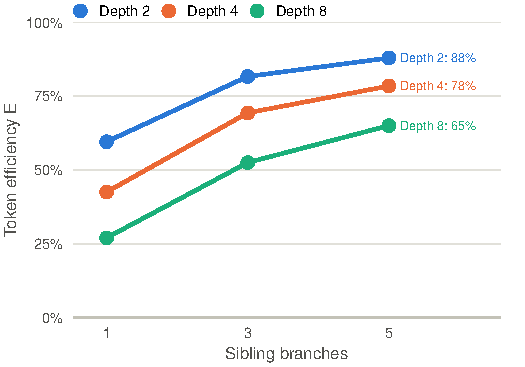
\includegraphics[width=\columnwidth]{fig3_efficiency.pdf}
\caption{Token efficiency of ancestor-only over full tree by sibling count and active-path depth (80 scenarios per point, 95\% intervals).}
\label{fig:eff}
\end{figure}

\subsection{Sibling Leakage}

Consistent with Proposition~\ref{prop:nosib}, ancestor-only prompting produced no leakage in 2{,}160 answers (exact 95\% upper bound 0.17\%), and no answer under any rule used an irrelevant sibling's detail. The baselines, by contrast, leaked from every other sibling type, as Fig.~\ref{fig:leak} shows. With consistent siblings, the full tree leaked in 32.4\% of answers and the window in 25.4\%. With conflicting siblings the order reversed, at 15.6\% and 38.5\%, and misleading siblings leaked least, at 3.3\% and 8.5\%.

\begin{figure}[t]
\centering
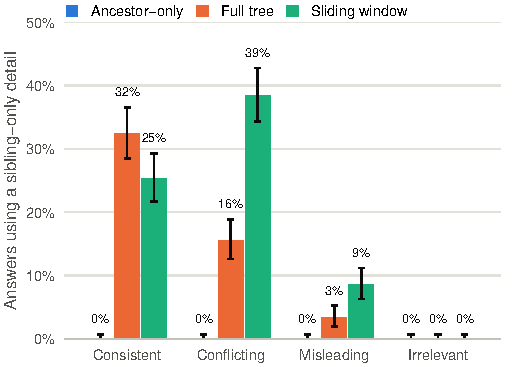
\includegraphics[width=\columnwidth]{fig1_leakage.pdf}
\caption{Answers that used a detail found only in an inactive branch, by sibling type and rule (judge-confirmed, about 540 answers per bar, exact 95\% intervals).}
\label{fig:leak}
\end{figure}

The mixed model confirms these differences after accounting for the other variables. The window leaked more than the full tree for conflicting siblings (model-based risk difference $+25.5$ points, 95\% CI $[+20.2,+30.7]$, Holm $p<10^{-20}$) and for misleading siblings ($+2.7$ $[+1.2,+4.2]$, $p<0.001$), but less for consistent siblings ($-8.2$ $[-13.6,-2.8]$, $p=0.003$). The conflicting case stands out most clearly once exposure is taken into account: when a conflicting value was in the prompt, models adopted it in 7.5\% of full-tree answers but in 86.9\% of window answers. Leakage also rose with depth (odds ratio 7.96 for depth 8 against depth 2) and with late siblings (2.70), and it was lower for GPT-6.2 Sol and Mistral Large 4 than for Gemini 4 Argon (odds ratios 0.12 and 0.13).

These rates depend on separating use from mention, since string matching alone overstates leakage (Fig.~\ref{fig:terms}). Of the 1{,}455 sibling terms found in full-tree answers, only 23.5\% were used; 49.2\% were mentioned only as alternatives that had not been chosen, and 26.0\% were explicitly rejected. In the window, by contrast, 65.0\% of the 837 flagged terms were used.

\begin{figure}[t]
\centering
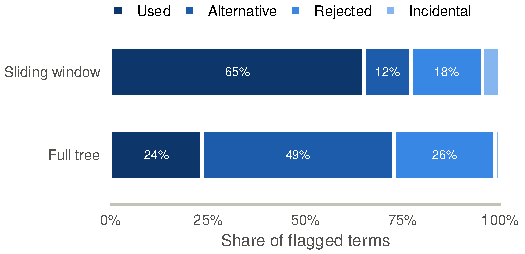
\includegraphics[width=\columnwidth]{fig2_term_usage.pdf}
\caption{How the judge labelled each sibling term found in an answer.}
\label{fig:terms}
\end{figure}

\subsection{Correctness and Quality}

Leakage did not always cost correctness, but losing the required fact did. Ancestor-only answers were correct in 99.9\% of cases, the full tree in 98.6\% and the window in only 52.0\% (Fig.~\ref{fig:correct}), and the same pattern held for all three models. Under the stricter string-only rule the figures fall to 99.1\%, 86.8\% and 50.5\%. The gap is largest for the full tree because most of its apparent errors were answers that stated the correct value and named a sibling's value only as an alternative.

\begin{figure}[t]
\centering
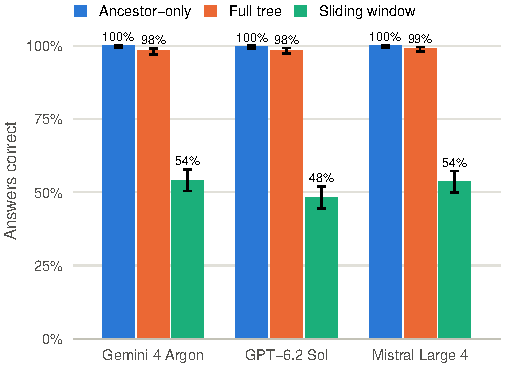
\includegraphics[width=\columnwidth]{fig4_correctness.pdf}
\caption{Correctness by model and rule (about 720 answers per bar, exact 95\% intervals).}
\label{fig:correct}
\end{figure}

The judge's quality scores followed the same order on every criterion (Table~\ref{tab:quality}). The full tree's largest loss was in contextual faithfulness ($-0.85$ points), which reflects answers that brought in details and alternatives from abandoned branches. The window lost far more on every criterion, most of all on faithfulness ($-2.51$ points on a 5-point scale).

\begin{table}[t]
\centering
\caption{Mean under ancestor-only and paired difference of each other rule from it (scenario $\times$ model pairs, bootstrap 95\% CI; Holm-adjusted $p<10^{-6}$ for all)}
\label{tab:quality}
\footnotesize
\setlength{\tabcolsep}{3pt}
\begin{tabular}{@{}lccc@{}}
\toprule
Measure & Ancestor & Full tree & Window \\
\midrule
Correct (\%) & 99.9 & $-1.3$ $[-1.9,-0.7]$ & $-47.9$ $[-51.7,-44.4]$ \\
Strict (\%) & 99.1 & $-12.4$ $[-14.5,-10.4]$ & $-48.7$ $[-52.1,-45.1]$ \\
Faithful. & 4.78 & $-0.85$ $[-0.92,-0.78]$ & $-2.51$ $[-2.63,-2.39]$ \\
Instruct. & 4.72 & $-0.18$ $[-0.22,-0.15]$ & $-1.77$ $[-1.87,-1.66]$ \\
Task & 4.36 & $-0.30$ $[-0.34,-0.27]$ & $-1.94$ $[-2.05,-1.83]$ \\
\bottomrule
\end{tabular}
\end{table}

\subsection{What the Window Displaces}

The window's losses follow directly from Propositions~\ref{prop:window} and \ref{prop:displace}. As Fig.~\ref{fig:window} shows, a root-side fact was never in the window (0 of 1{,}080 cases), whereas a current-turn fact with early siblings always was. With late siblings, the current-turn fact survived in only 16.1\% of cases, and these were exactly the cases in which the condition of Proposition~\ref{prop:displace} held. Whether the fact survived then decided the answer: correctness was 99.8\% when it did and 32.4\% when it was displaced. As a result, recency and fact position interacted strongly (difference-in-differences of $-67.6$ points in correctness, 95\% CI $[-78.8,-56.4]$).

\begin{figure}[t]
\centering
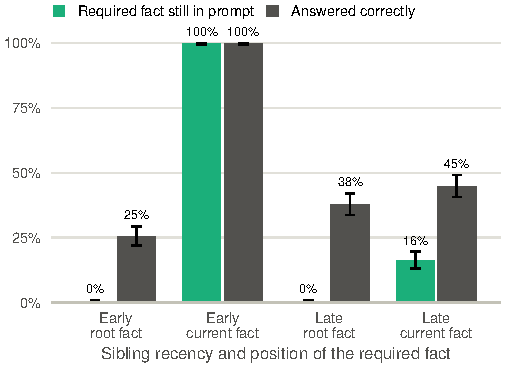
\includegraphics[width=\columnwidth]{fig6_window_displacement.pdf}
\caption{Sliding window only: share of prompts that still contained the required fact, and share of answers correct (about 540 per cell).}
\label{fig:window}
\end{figure}

\subsection{The Price of Ancestor-Only Prompting}

Consistent siblings are the one case in which sibling content can help, and so they measure what ancestor-only prompting gives up. In the full tree and the window, every answer that used a consistent detail was correct. The effect was largest where the window had already displaced the required fact: there, answers that used the consistent detail were correct in 100\% of cases ($n=107$), against 43.2\% for those that did not ($n=271$; Fisher exact $p<10^{-30}$), as Fig.~\ref{fig:consistent} shows. The judge nonetheless scored these answers lower on faithfulness ($-1.28$ points, $[-1.43,-1.12]$) and task completion ($-0.36$, $[-0.51,-0.22]$), because they presented details that were absent from the active path as if they had been agreed.

\begin{figure}[t]
\centering
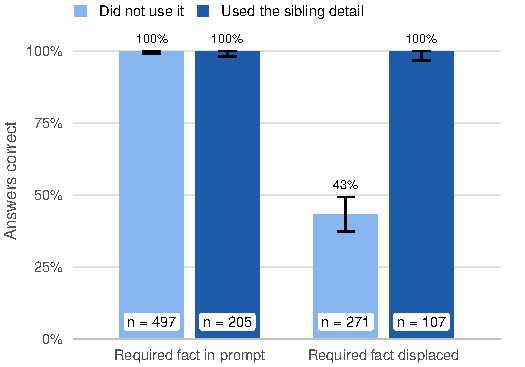
\includegraphics[width=\columnwidth]{fig7_consistent_price.pdf}
\caption{Answers with a consistent sibling (full tree and window), by whether the sibling's detail was used and whether the required fact was still in the prompt (exact 95\% intervals).}
\label{fig:consistent}
\end{figure}

\subsection{Robustness}

These results were stable across repeated runs. Across the 73 scenarios run three times, the leakage outcome was identical in all three runs in 91.8--100\% of cases and correctness in 91.8--100\%, depending on model and rule. Gemini 4 Argon's leakage was fully repeatable, and its correctness changed in a single full-tree scenario. Finally, Table~\ref{tab:theory} lists each formal prediction alongside its outcome; all of them held without exception.

\begin{table}[t]
\centering
\caption{Formal predictions checked against the full run}
\label{tab:theory}
\begin{tabular}{@{}lll@{}}
\toprule
Statement & Prediction & Observed \\
\midrule
Prop.~\ref{prop:eff} & $E=w(\Sib)/w(V)$ & exact in 720/720 \\
Prop.~\ref{prop:nosib} & no canary, ancestor-only & 0 of 2{,}598 \\
Prop.~\ref{prop:window} & which facts the window keeps & 720/720 \\
Prop.~\ref{prop:window} & root fact never kept & 0 of 360 cells \\
Prop.~\ref{prop:displace} & late-sibling survival & 360/360 \\
\bottomrule
\end{tabular}
\end{table}

\section{Discussion}

\textit{Research question.} At an equal token budget, selecting context by tree structure rather than by recency removed sibling leakage entirely and preserved answer quality on the active path, while the window lost about half of its correct answers. Each part of the hypothesis therefore held: ancestor-only prompting used fewer tokens than the full tree, both baselines leaked, and quality was preserved whenever the required fact lay on the active path.

\textit{Results against expectation.} Given the literature on long context, one might expect the full tree, the longest prompt, to perform worst. Instead, it was nearly as accurate as ancestor-only prompting (98.6\% against 99.9\%) and far more accurate than the much shorter window. Its costs lay elsewhere, in three times the tokens, in leakage and in lower judged quality. The window, in turn, failed less because of its length than because of \emph{which} tokens it kept. It discards the oldest active messages first, and once the decision is gone, a conflicting sibling supplies the only available answer, which models adopted in 86.9\% of exposed cases. Length alone therefore does not explain the advantage of ancestor-only prompting, which is the question that prior work \cite{nanjundappa2025branching} left open.

\textit{Consistent siblings.} This leaves the question of what ancestor-only prompting gives up. Its price is measurable only when a consistent sibling carries information that the prompt has otherwise lost, and in this benchmark that happened only after the window displaced the required fact. Under ancestor-only prompting the required fact is always present, so the price never cost it a correct answer. In real use, however, a consistent sibling may hold a fact that is useful but was never stated on the active path, and such cases would need retrieval across branches.

\textit{Limitations.} Several limitations qualify these findings. The scenarios are synthetic and template-based, with forced-choice answers, so absolute rates may not transfer to free-form conversations. Only three models were tested; one of them (GPT-6.2 Sol) could not be run at temperature 0, and Mistral Large 4 was not fully deterministic. Quality scores come from a single LLM judge whose rubric penalizes details absent from the active path even when they are true, and its agreement with human scores is reported in Section~IV-C \todo{update}. Correctness likewise relies on the leak judge to separate asserted from merely mentioned values, which is why the stricter string-only rule is reported alongside it. Finally, window leakage was measured only where a planted item was exposed; this is the quantity Proposition~\ref{prop:decomp} identifies, but it covers fewer calls than in the full tree.

\section{Conclusion}

Choosing context by tree structure made branched conversations 62.7\% cheaper than full-tree concatenation and free of sibling leakage, without any loss of quality on the active path. A recency window of the same size, by contrast, lost root-side facts and adopted conflicting siblings in their place. Tree structure alone is therefore a sound basis for deciding what a branching chat tool sends to the model on each turn. Where a needed fact lives outside the active path, future work could combine that path with selective retrieval from sibling branches.

\section*{Reproducibility}
The generator, frozen dataset (sha256 \texttt{4c3e5380\ldots c37d}), raw model responses, judge outputs and analysis scripts are available on the \texttt{thesis/experiment} branch of the Traceback repository, tag \texttt{thesis-freeze-v1}. The total model and judge cost was US\$86.11.

% \section*{Use of AI Tools}
% \todo{Disclose AI assistance according to your department's policy.}

\begin{thebibliography}{99}

\bibitem{hong2025contextrot}
K. Hong, A. Troynikov, and J. Huber, ``Context rot: How increasing input tokens impacts LLM performance,'' Chroma, Tech. Rep., Jul. 2025. [Online]. Available: \url{https://research.trychroma.com/context-rot}

\bibitem{liu2024lost}
N. F. Liu, K. Lin, J. Hewitt, A. Paranjape, M. Bevilacqua, F. Petroni, and P. Liang, ``Lost in the middle: How language models use long contexts,'' \emph{Trans. Assoc. Comput. Linguistics}, vol. 12, pp. 157--173, 2024.

\bibitem{hemanth2026cta}
P. Hemanth and S. Saha, ``Conversation tree architecture: A structured framework for context-aware multi-branch LLM conversations,'' arXiv:2603.21278, 2026. [Online]. Available: \url{https://arxiv.org/abs/2603.21278}

\bibitem{nanjundappa2025branching}
B. Chickmagalur Nanjundappa and S. Maaheshwari, ``Context branching for LLM conversations: A version control approach to exploratory programming,'' arXiv:2512.13914, Dec. 2025. [Online]. Available: \url{https://arxiv.org/abs/2512.13914}

\bibitem{jiang2024longllmlingua}
H. Jiang, Q. Wu, X. Luo, D. Li, C.-Y. Lin, Y. Yang, and L. Qiu, ``LongLLMLingua: Accelerating and enhancing LLMs in long context scenarios via prompt compression,'' in \emph{Proc. 62nd Annu. Meeting Assoc. Comput. Linguistics (ACL)}, 2024.

\bibitem{zheng2023judging}
L. Zheng \emph{et al.}, ``Judging LLM-as-a-judge with MT-Bench and Chatbot Arena,'' in \emph{Advances in Neural Information Processing Systems (NeurIPS), Datasets and Benchmarks Track}, 2023.

\bibitem{cohen1960kappa}
J. Cohen, ``A coefficient of agreement for nominal scales,'' \emph{Educ. Psychol. Meas.}, vol. 20, no. 1, pp. 37--46, 1960.

\bibitem{bates2015lme4}
D. Bates, M. M\"achler, B. Bolker, and S. Walker, ``Fitting linear mixed-effects models using lme4,'' \emph{J. Stat. Softw.}, vol. 67, no. 1, pp. 1--48, 2015.

\bibitem{clopper1934}
C. J. Clopper and E. S. Pearson, ``The use of confidence or fiducial limits illustrated in the case of the binomial,'' \emph{Biometrika}, vol. 26, no. 4, pp. 404--413, 1934.

\bibitem{lenth2025emmeans}
R. V. Lenth, ``emmeans: Estimated marginal means, aka least-squares means,'' R package version 2.0.4, 2026.

\bibitem{wilcoxon1945}
F. Wilcoxon, ``Individual comparisons by ranking methods,'' \emph{Biometrics Bull.}, vol. 1, no. 6, pp. 80--83, 1945.

\bibitem{efron1993bootstrap}
B. Efron and R. J. Tibshirani, \emph{An Introduction to the Bootstrap}. New York, NY, USA: Chapman \& Hall, 1993.

\bibitem{holm1979}
S. Holm, ``A simple sequentially rejective multiple test procedure,'' \emph{Scand. J. Statist.}, vol. 6, no. 2, pp. 65--70, 1979.

\end{thebibliography}

\end{document}
